%! Author = gramic
%! Date = 29.04.24

% Preamble
\begin{flushleft}
    \subsection{Architektur}
    Das Testsystem wird mit Patroni umgesetzt.\\
    Dabei werden folgende Komponenten eingesetzt:\\
    \begin{longtable}[H]{ll}

\toprule
Aufgabe & System \\
\midrule
\endfirsthead
\caption[]{Testsystem - Komponenten} \\
\toprule
Aufgabe & System \\
\midrule
\endhead
\midrule
\multicolumn{2}{r}{Continued on next page} \\
\midrule
\endfoot
\bottomrule
\endlastfoot
Orchestrator & Patroni \\
Proxy & Haproxy \\
\Gls{Connection Pooler} & PgBouncer \\
\Gls{DCS} & \gls{etcd} \\
\caption{Testsystem - Komponenten} \label{construction_components}
\end{longtable}

\end{flushleft}
\begin{flushleft}
    Entsprechend sieht das Architekturschema aus:
    \begin{figure}[H]
        \centering
        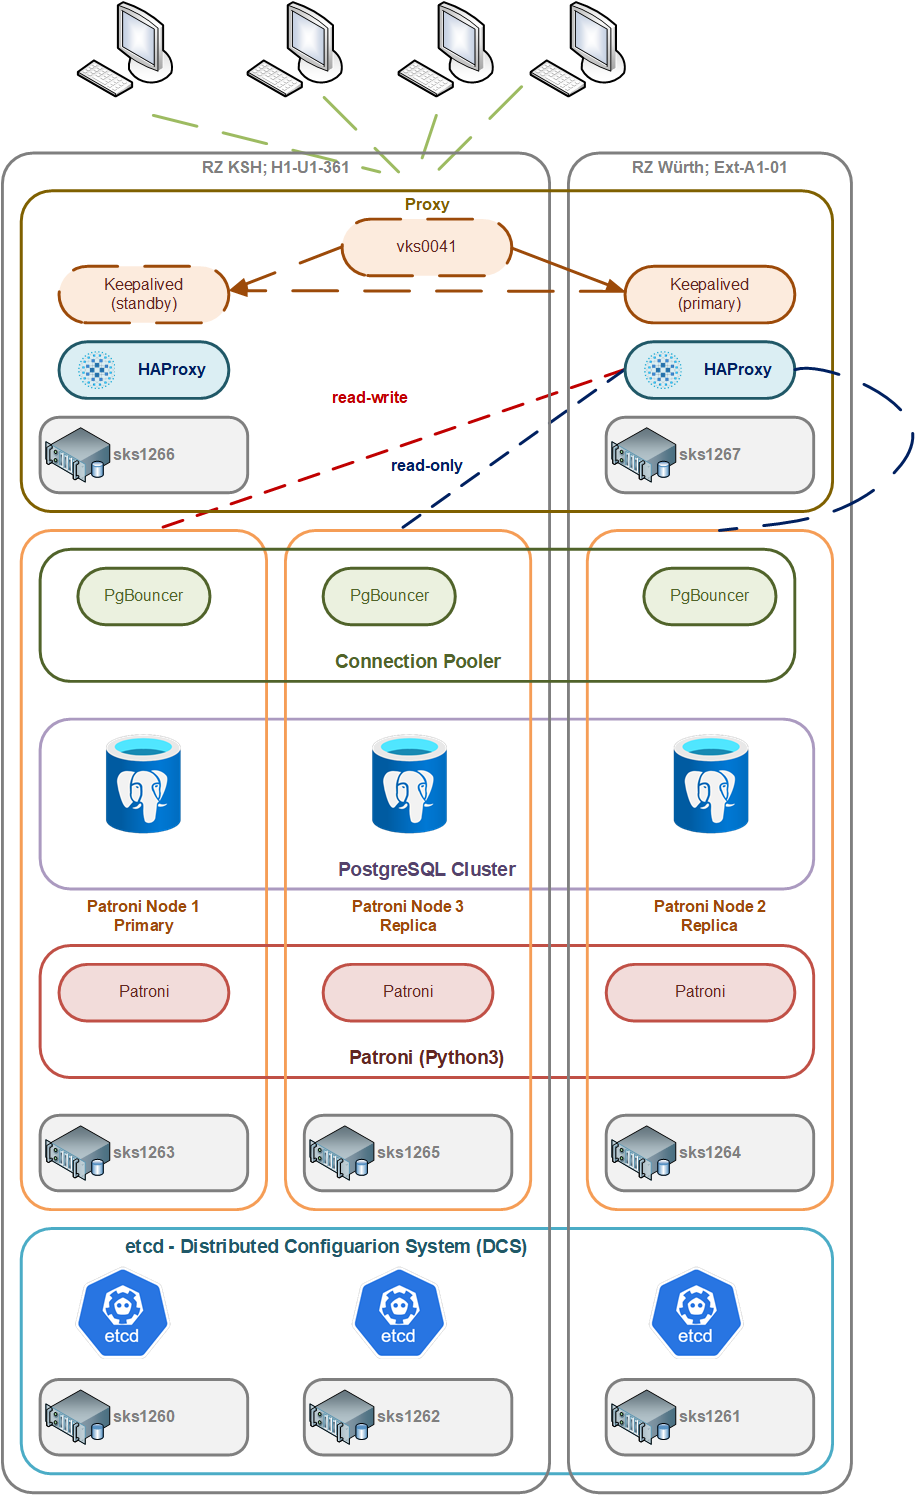
\includegraphics[width=0.75\linewidth]{source/implementation/construction_implementation/patroni-construction-architecture}
        \caption{Testsystem - Architektur}
        \label{fig:patroni-construction-architecture}
    \end{figure}
\end{flushleft}
\begin{flushleft}
    \texttt{vitabacks / postgresql\_cluster} hat eine Schwachstelle.\\
    Der \Gls{Connection Pooler} ist nicht auf dem Level des Proxy sondern auf dem Patroni Node.\\
    Das Resultat bei einem Node Failure ist zwangsläufig, dass die Connections bei einem \Gls{Switchover} / \Gls{Failover} unterbrochen werden.\\
    Sollte die Applikation nicht fähig sein, die Connection zu halten und innerhalb eines Timeouts reconnecten zu können,\\
    kommt es zu einem Finalen Disconnect.\\
    Ohne weiteres lässt sich der \Gls{Connection Pooler} aber nicht auf den Proxy-Server verschieben, zu tief müsste in den Code eingegriffen werden.
\end{flushleft}